\chapter{Sums of Combinatorial Games}
\marginurl{%
    Sum of Games:\\\noindent
    Introduction to Combinatorial Game Theory \#5
}{youtu.be/dRaqJKZh3y0}


Let us consider the following game.
\begin{game}[Take-Away Game]
\label{game:two-pile-take-away-n-m-2-1}
  In this game there are two players.
  \begin{itemize}
    \item They have two piles of $n$ and $m$ chips, respectively.
    \item They make moves in turns with player I starting,
      each move consists of moving one or two chips out of the pile.
    \item The player that removes the last chip wins.
  \end{itemize}
\end{game}
It is not hard to draw the graph corresponding to the game for small $n$ and
$m$.
\begin{figure}
  \centering
  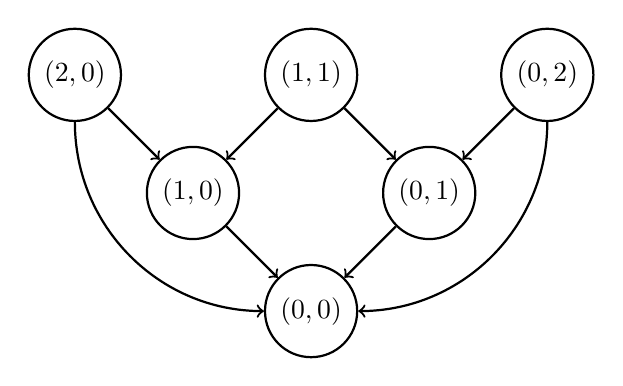
\begin{tikzpicture}[thick]
    \node[circle, draw, minimum size=6pt] (v1) at (0,0) {$(0, 0)$};
    \node[circle, draw, minimum size=6pt] (v2) at (1.5,1.5) {$(0, 1)$};
    \node[circle, draw, minimum size=6pt] (v3) at (-1.5,1.5) {$(1, 0)$};
    \node[circle, draw, minimum size=6pt] (v4) at (0,3) {$(1, 1)$};
    \node[circle, draw, minimum size=6pt] (v5) at (3,3) {$(0, 2)$};
    \node[circle, draw, minimum size=6pt] (v6) at (-3,3) {$(2, 0)$};


    \draw[->] (v2) -- (v1);
    \draw[->] (v3) -- (v1);
    \draw[->] (v4) -- (v2);
    \draw[->] (v4) -- (v3);
    \draw[->] (v5) to[out=-90, in=0] (v1);
    \draw[->] (v6) to[out=-90, in=180] (v1);
    \draw[->] (v6) -- (v3);
    \draw[->] (v5) -- (v2);
  \end{tikzpicture}
  \caption{Part of the graph of \Cref{game:two-pile-take-away-n-m-2-1}}
\end{figure}
Using this graph it is easy to see that all drawn positions, except $(1, 1)$ and
$(0, 0)$ are N-positions.

In the rest of the chapter we will discuss a method to study similar games.
Assume we have two combinatorial games $\mathcal{G}_1$ and $\mathcal{G}_2$.
One may form another game played as follows: the initial position of the new game
consists of the pair of initial positions of $\mathcal{G}_1$ and $\mathcal{G}_2$,
players alternate moves, and on each turn a player make a move in one of the game
leaving the position in the second untouched.  The new game is called
\emph{sum of $\mathcal{G}_1$ and $\mathcal{G}_2$}.

Let us give a formal definition.
\begin{definition}
    Let $G_1 = (V_1, F_1)$ and $G_2 = (V_1, F_2)$ be directed graphs.
    We say that $G$ is the sum of $G_1$ and $G_2$, denoted $G_1 + G_2$, is
    a graph $(V_1 \times V_2, F)$  such that
    \[
        F(x_1, x_2) =
            \set[y_1 \in F_1(x_1)]{(y_1, x_2)} \cup
            \set[y_2 \in F_2(x_2)]{(x_1, y_2)}.
    \]
\end{definition}
\Cref{figure:sum-of-graphs-G1-G2} gives an example of this operation.

\begin{figure}
    \centering
    \subfloat[$G_1$\label{figure:sum-of-graphs-G1}]{
        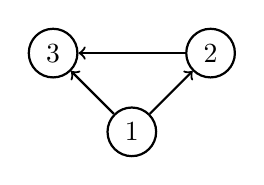
\begin{tikzpicture}[thick]
          \node[circle, draw, minimum size=6pt] (v1) at (0,0) {$1$};
          \node[circle, draw, minimum size=6pt] (v2) at (1,1) {$2$};
          \node[circle, draw, minimum size=6pt] (v3) at (-1,1) {$3$};


          \draw[->] (v1) -- (v2);
          \draw[->] (v1) -- (v3);
          \draw[->] (v2) -- (v3);
        \end{tikzpicture}
    }
    \qquad\qquad
    \subfloat[$G_2$\label{figure:sum-of-graphs-G2}] {
        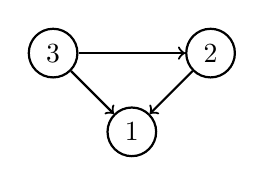
\begin{tikzpicture}[thick]
          \node[circle, draw, minimum size=6pt] (v1) at (0,0) {$1$};
          \node[circle, draw, minimum size=6pt] (v2) at (1,1) {$2$};
          \node[circle, draw, minimum size=6pt] (v3) at (-1,1) {$3$};


          \draw[->] (v2) -- (v1);
          \draw[->] (v3) -- (v1);
          \draw[->] (v3) -- (v2);
        \end{tikzpicture}
    }
    \qquad\qquad
    \subfloat[$G_1 + G_2$\label{figure:sum-of-graphs-G1-G2}] {
        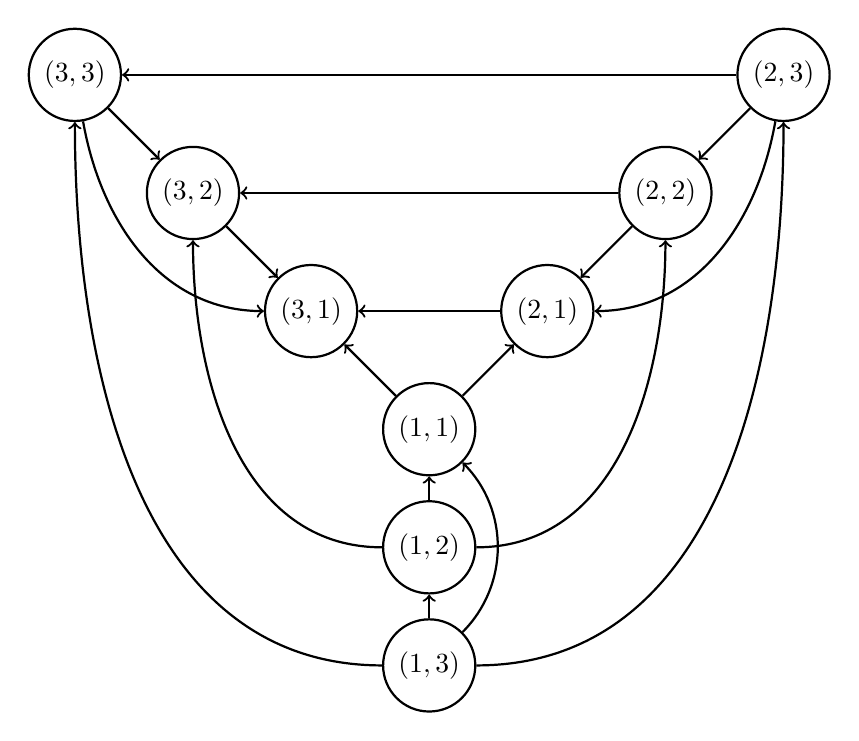
\begin{tikzpicture}[thick]
          \node[circle, draw, minimum size=6pt] (v11) at (0, 0)  {$(1, 1)$};
          \node[circle, draw, minimum size=6pt] (v21) at (1.5, 1.5)  {$(2, 1)$};
          \node[circle, draw, minimum size=6pt] (v31) at (-1.5, 1.5) {$(3, 1)$};
          \node[circle, draw, minimum size=6pt] (v12) at (0, -1.5) {$(1, 2)$};
          \node[circle, draw, minimum size=6pt] (v22) at (3, 3)  {$(2, 2)$};
          \node[circle, draw, minimum size=6pt] (v32) at (-3, 3) {$(3, 2)$};
          \node[circle, draw, minimum size=6pt] (v13) at (0,-3)  {$(1, 3)$};
          \node[circle, draw, minimum size=6pt] (v23) at (4.5,4.5)  {$(2, 3)$};
          \node[circle, draw, minimum size=6pt] (v33) at (-4.5,4.5) {$(3, 3)$};


          \draw[->] (v11) -- (v21);
          \draw[->] (v11) -- (v31);
          \draw[->] (v21) -- (v31);
          \draw[->] (v12) to[out = 0, in = -90] (v22);
          \draw[->] (v12) to[out = 180, in = -90] (v32);
          \draw[->] (v22) -- (v32);
          \draw[->] (v13) to[out = 0, in = -90] (v23);
          \draw[->] (v13) to[out = 180, in = -90] (v33);
          \draw[->] (v23) -- (v33);
          \draw[->] (v12) -- (v11);
          \draw[->] (v13) to[out = 45, in = -45] (v11);
          \draw[->] (v13) -- (v12);
          \draw[->] (v22) -- (v21);
          \draw[->] (v23) to[out = -100, in = 0] (v21);
          \draw[->] (v23) -- (v22);
          \draw[->] (v32) -- (v31);
          \draw[->] (v33) to[out = -80, in = 180] (v31);
          \draw[->] (v33) -- (v32);
        \end{tikzpicture}
    }
    \caption{\Cref{figure:sum-of-graphs-G1-G2} depicts sum of graphs
        from \Cref{figure:sum-of-graphs-G1} and \Cref{figure:sum-of-graphs-G2}.
    }
\end{figure}


Another example is given by the game of Nim; it is easy to see that
$2$-pile Nim is a sum of two $1$-pile Nims. This observation leads to a
generalization of Bouton's Theorem (\Cref{theorem:bouton}).
\begin{theorem}[The Sprague--Grundy Theorem]
    Let $G_1$ and $G_2$ be some graphs and $g_1$ and $g_2$ be corresponding
    Sprague--Grundy functions. Then the graph $G_1$ and $G_2$ has a
    Sprague--Grundy function $g$ such that
    $g(x_1, x_2) = g_1(x_1) \bitwisexor g_2(x_2)$.
\end{theorem}
\begin{proof}
    Let $G_1 = (V_1, F_1)$, $G_2 = (V_2, F_2)$, and $G = G_1 + G_2$.
    Consider some $x_1 \in V_1$ and $x_2 \in V_2$.
    Let $a = g_1(x_1) \bitwisexor g_2(x_2)$. To prove the statement we need to
    show that
    \begin{enumerate}
        \item for any $0 \le b < a$, there is $(y_1, y_2) \in F(x_1, x_2)$ such
            that $g(y_1, y_2) = b$;
        \item for any $(y_1, y_2) \in F(x_1, x_2)$, $g(y_1, y_2) \neq a$.
    \end{enumerate}

    We start from proving the first statement.
    Let us fix some $0 \le b < a$ and let $c = a \bitwisexor b$.
    Let $g_i(x_i) = (p_{i, \ell}, \dots, p_{i, 0})$ for each $i \set{1, 2}$ and
    $c = (1, q_{k - 1}, \dots, q_0)$ where $k \le \ell$.
    For some $j \in \set{1, 2}$, $p_{j, k} = 1$ since
    $a = g_1(x_1) \bitwisexor g_2(x_2)$. Without loss of generality $j = 1$.
    Hence, $c \bitwisexor g_1(x_1) < g_1(x_1)$, whence there is $x'_1$ such
    that $g_1(x'_1) = c \bitwisexor g_1(x_1)$. As a result, there is a move in
    $G$ from $(x_1, x_2)$ to $(x'_1, x_2)$ and
    $g(x'_1, x_2) = g_1(x'_1) \bitwisexor g_2(x_2) =
        c \bitwisexor g_1(x_1) \bitwisexor g_2(x_2) =
        c \bitwisexor a = b$.

    To prove the second statement, assume that there is
    $(y_1, y_2) \in F(x_1, x_2)$ so that $g(y_1, y_2) = a$. Without loss of
    generality we may assume that $x_2 = y_2$. Hence,
    $0 = g(y_1, x_2) \bitwisexor g(x_1, x_2) = g_1(y_1) \bitwisexor g_1(x_1)$.
    However, $g_1(y_1) \neq g_1(x_1)$ since there is a move from $x_1$ to $y_1$.
    Therefore $g_1(y_1) \bitwisexor g_1(x_1) \neq 0$ which is a contradiction.
\end{proof}
It is also easy to see that if $G_1$ and $G_2$ satisfy the ending condition,
then $G_1 + G_2$ also satisfies the ending condition. Therefore, if $G_1$ and
$G_2$ satisfy the ending condition and $g_1$, $g_2$ are Sprague--Grundy
functions of them, $G_1 + G_2$ has unique Sprague--Grundy function $g$ such that
$g(x_1, x_2) = g_1(x_1) \bitwisexor g_2(x_2)$.

The simple example of an application of this theorem is the analysis of the
following game.
\begin{game}
\label{game:subtraction-1-2-3-out-of-10-11}
  Alice and Bob have two piles with $10$ and $11$ chips respectively.
  They take turns and remove $1$ or $2$ chips from one of the piles.
  If one of them cannot make a move he/she loses.
\end{game}

To determine who is the winner in this game, we start with a subtraction game
$G$ with the subtraction set $\set{1, 2}$. It is easy to see that 
$g : \N_0 \to \N_0$ such that
\[
  g(x) =
  \begin{cases}
    0 & \text{if } x \equiv 0 \pmod{3} \\
    1 & \text{if } x \equiv 1 \pmod{3} \\
    2 & \text{if } x \equiv 2 \pmod{3}
  \end{cases}
\]
is the Sprague--Grundy function for $G$. 
It is also clear that \Cref{game:subtraction-1-2-3-out-of-10-11} is equal to 
$G + G$. Therefore the function $g' : \N_0^2 \to \N_0$ such that 
\[
  g(x, y) =
  \begin{cases}
    0 & \text{if } x \equiv 0 \pmod{3} \text{ and } y \equiv 0 \pmod{3}\\
    1 & \text{if } x \equiv 0 \pmod{3} \text{ and } y \equiv 1 \pmod{3}\\
    2 & \text{if } x \equiv 0 \pmod{3} \text{ and } y \equiv 2 \pmod{3}\\
    1 & \text{if } x \equiv 1 \pmod{3} \text{ and } y \equiv 0 \pmod{3}\\
    0 & \text{if } x \equiv 1 \pmod{3} \text{ and } y \equiv 1 \pmod{3}\\
    3 & \text{if } x \equiv 1 \pmod{3} \text{ and } y \equiv 2 \pmod{3}\\
    2 & \text{if } x \equiv 2 \pmod{3} \text{ and } y \equiv 0 \pmod{3}\\
    3 & \text{if } x \equiv 2 \pmod{3} \text{ and } y \equiv 1 \pmod{3}\\
    0 & \text{if } x \equiv 2 \pmod{3} \text{ and } y \equiv 2 \pmod{3}
  \end{cases}
\]
Therefore, the position $(10, 11)$ is an N-position.


\marginurl{%
    Applications of the Sprague-Grundy Theorem:\\\noindent
    Introduction to Combinatorial Game Theory \#6
}{youtu.be/V4yI_1P1Jcc}
A surprising example of the application of this theorem is the following game.
\begin{game}
\label{game:polygon}
  In this game position is described by a polygon with several diagonals. 
  The game starts with a polygon with $n$ sides. On each turn a player draw a
  new diagonal so that it does not intersect with previously drawn diagonals.
  Players take turns and the one who cannot make a move loses.
\end{game}
It is easy to see that we do not care about the shape of the polygon and
diagonals, the only important information is the number of nodes and which nodes
are connected by a diagonal. 

Let $g(n)$ be the value of the Sprague--Grundy function at the polygon with $n$
sides. It is easy to see that if we split the polygon, by a diagonal, into two
parts with $\ell$ and $m$ sides, then the resulting position is essentially a
position in the sum of two games; 
hence, 
$g(n) = 
  \mex \set[
    \ell, m \ge 3 \text{ and } \ell + m = n + 2
  ]{g(\ell) \bitwisexor g(m)}$.
Using this observation it is easy to compute the value of $g(n)$ for small $n$.
\begin{table}[h!]
  \centering
  \begin{tabular}{l l l l l l l l l}
      \toprule
      3 & 4 & 5 & 6 & 7 & 8 \\
      \midrule
      0 & 1 & 0 & 1 & 0 & 1 \\
      \bottomrule
  \end{tabular}
  \caption{Sprague--Grundy function for \Cref{game:polygon}}
\end{table}
It is easy to see to make a conjecture that $g(n) = 0$ for odd $n$ and $g(n) =
1$ for even $n$. Let us prove this using induction. The base case follows from
the computation necessary to write the table. Let us prove the induction step
from $1, \dots, n$ to $n + 1$.
\begin{itemize}
  \item Let $n + 1$ be even. It is clear that if $\ell + m = (n + 1) + 2$, then
    $\ell$ and $m$ have the same remainder modulo $2$. Therefore, $g(m) =
    g(\ell)$ by the induction hypothesis. As a result, 
    \[
      \set[
        \ell, m \ge 3 \text{ and } \ell + m = n + 2
      ]{g(\ell) \bitwisexor g(m)} = \set{0}
    \] 
    and $g(n + 1) = 1$.    
  \item Let $n + 1$ be odd. It is clear that if $\ell + m = (n + 1) + 2$, then
    $\ell$ and $m$ have different remainders modulo $2$. Therefore, $g(m) \neq
    g(\ell)$ by the induction hypothesis. As a result, 
    \[
      \set[
        \ell, m \ge 3 \text{ and } \ell + m = n + 2
      ]{g(\ell) \bitwisexor g(m)} = \set{1}
    \] 
    and $g(n + 1) = 0$.
\end{itemize}
\begin{chapterendexercises}
    \exercise Compute the Sprague--Grundy function for states of the subtraction
      game with two piles of chips where players and the subtraction set 
      $\set{1, 2, 5}$.
    \exercise Let $G_1$ be the subtraction game with the subtraction set
      $\set{1, 2}$
      Let $G_2$ be the game of Nim with three piles.
      Find all the moves from $(11, (1, 6, 7))$ to P-positions in 
      $G1 + G2$.
\end{chapterendexercises}
